\documentclass{article}
\usepackage[utf8]{inputenc}
\usepackage{listings}
\usepackage[top=100pt,right=100pt,bottom=100pt,left=100pt, includefoot, includehead]{geometry}
\usepackage{xcolor}
\usepackage{textcomp}
\usepackage{color}
\usepackage[T1]{fontenc}
\usepackage{float}
\usepackage{graphicx}

\title{Baza danych biblioteki\\\large Projekt zaliczeniowy z przedmiotu Bazy Danych}
\author{Mateusz Winiarski}
\date{1 lutego 2023}

\definecolor{codegreen}{rgb}{0,0.6,0}
\definecolor{codegray}{rgb}{0.5,0.5,0.5}
\definecolor{codepurple}{HTML}{C42043}
\definecolor{backcolour}{HTML}{F2F2F2}
\definecolor{bookColor}{cmyk}{0,0,0,0.90}  
\color{bookColor}

\lstset{upquote=true}

\lstdefinestyle{mystyle}{
    backgroundcolor=\color{backcolour},   
    commentstyle=\color{codegreen},
    keywordstyle=\color{codepurple},
    numberstyle=\numberstyle,
    stringstyle=\color{codepurple},
    basicstyle=\footnotesize\ttfamily,
    breakatwhitespace=false,
    breaklines=true,
    captionpos=b,
    keepspaces=true,
    numbers=left,
    numbersep=10pt,
    showspaces=false,
    showstringspaces=false,
    showtabs=false,
}
\lstset{style=mystyle}

\newcommand\numberstyle[1]{%
    \footnotesize
    \color{codegray}%
    \ttfamily
    \ifnum#1<10 0\fi#1 |%
}

\renewcommand\t\texttt

\begin{document}

\maketitle

\section{Założenia}

\subsection{Zadanie bazy danych}
Celem projektu jest stworzenie bazy danych dla biblioteki ułatwiającej zarządzanie pozycjami, użytkownikami biblioteki oraz wypożyczeniami. 

Baza zawiera podstawowe tabele zawierające najbardziej podstawowe dane o pozycjach, książkach, użytkownikach i wypożyczeniach. System może być łatwo rozbudowany o nowe funkcjonalności. W praktyce można umieścić w bazie dużo więcej informacji o książkach, użytkownikach, czy autorach książek.


\subsection{Lista tabel}

\begin{itemize}
    \item \t{Items}
    \item \t{Books}
    \item \t{Other}
    \item \t{Authors}
    \item \t{Redactors}
    \item \t{Categories}
    \item \t{CategoryTree}
    \item \t{Users}
    \item \t{Borrowings}
    \item \t{Fines}
\end{itemize}

\subsection{Diagram ER}

\begin{figure}[H]
    \centering
    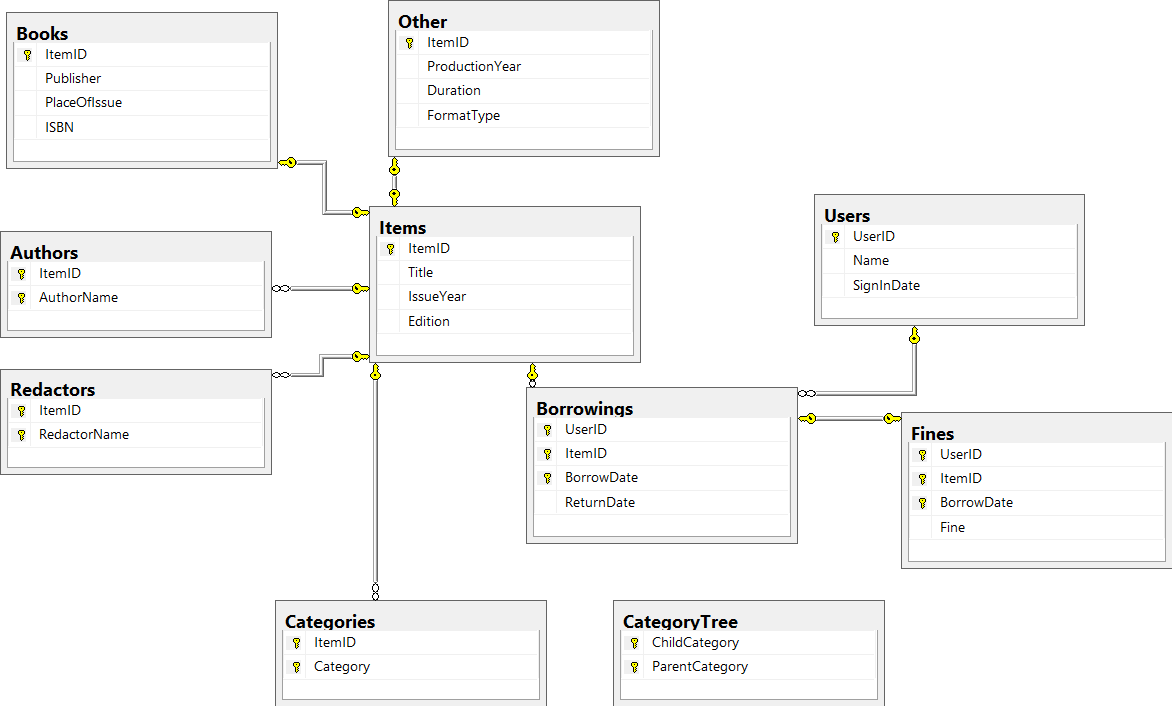
\includegraphics[width=\textwidth]{diergram.png}
    \caption{Diagram ER}
    \label{er}
\end{figure}

\subsection{Schemat bazy danych}

\begin{figure}[H]
    \centering
    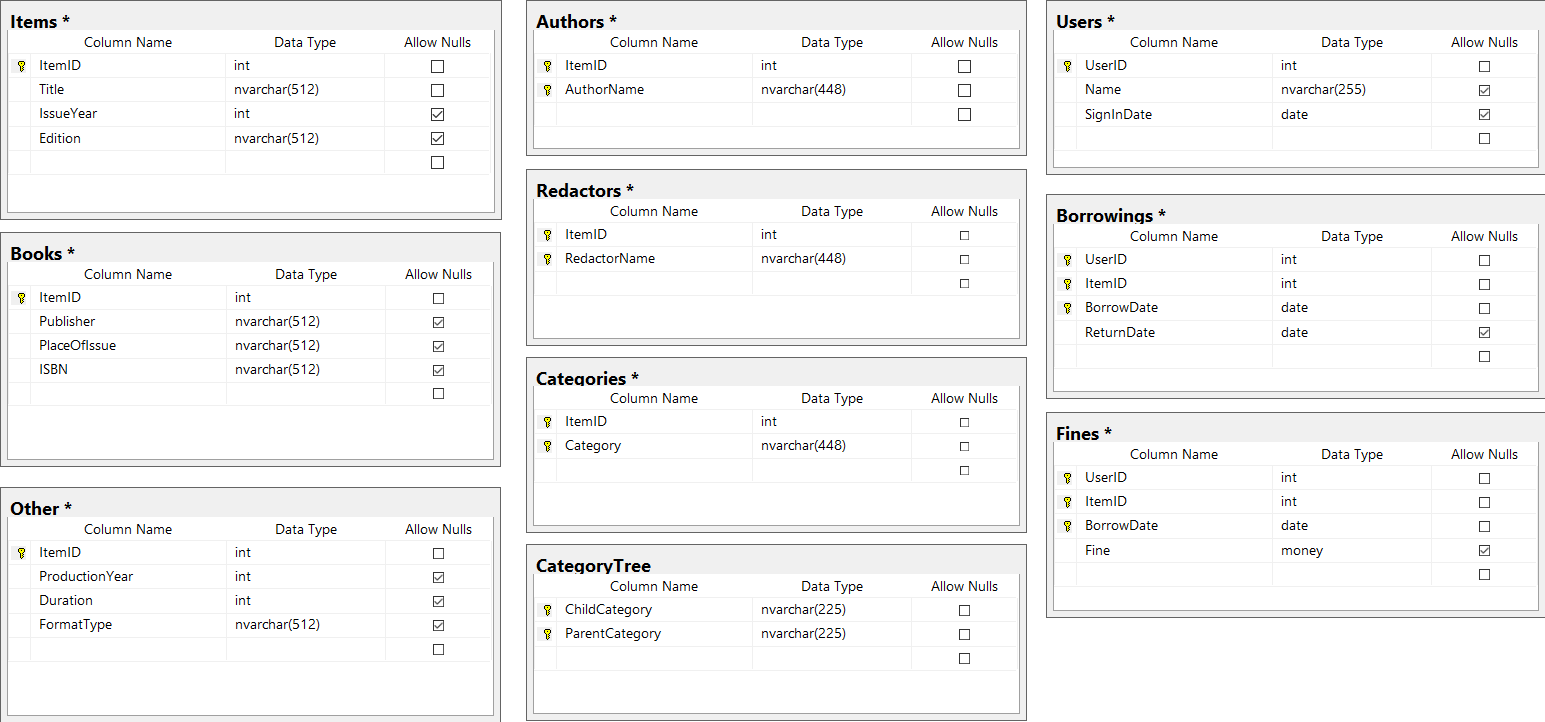
\includegraphics[width=\textwidth]{schemgram.png}
    \caption{Schemat bazy danych}
    \label{sb}
\end{figure}

\subsection{Konserwacja bazy danych}

Baza danych powinna być często backupowana, ze względu na częste zmiany informacji i ilość pracy, jaka została włożona w spisanie danych wszystkich pozycji. Zapasowa kopia przyrostowa powinna być robiona codziennie (najlepiej w godzinach zamknięcia biblioteki), natomiast kopia calościowa co tydzień.


\section{Zapytania}

Do bazy danych napisane jest 10 widoków, 5 procedur oraz 5 wyzwalaczy.

\subsection{Widoki}

Widoki pozwalają na zobaczenie najczęściej wyświetlanych i najbardziej ogólnych zestawień, takich jak ogólnodostępne lista wszystkich książek \t{AllBooks}, lista wszystkich innych pozycji \t{AllOther}, lista wszystkich autorów \t{CountByAuthor}, lista wszystkich kategorii \t{CountByCategory}, lista książek według dekady \t{CountByDecade} oraz statystyki książek \t{ItemBorrowingStats}, a także dostępne dla administratorów lista użytkowników \t{AllUsers}, lista naliczonych kar \t{AllFines}, lista wypożyczonych książek \t{CurrentlyBorrowedBooks} oraz licznik książek z brakami w danych \t{CountUncompleteBooks}.

\begin{lstlisting}[ language=SQL,
                    framesep=8pt,
                    xleftmargin=40pt,
                    framexleftmargin=40pt,
                    frame=tb,
                    framerule=0pt
                    ]
CREATE VIEW AllBooks AS
	SELECT I.Title, B.Publisher, I.IssueYear, B.PlaceOfIssue, I.Edition, B.ISBN FROM
	Items I JOIN Books B
	ON I.ItemID = B.ItemID
	ORDER BY I.Title OFFSET 0 ROWS
GO
\end{lstlisting}

\begin{lstlisting}[ language=SQL,
                    framesep=8pt,
                    xleftmargin=40pt,
                    framexleftmargin=40pt,
                    frame=tb,
                    framerule=0pt
                    ]
CREATE VIEW AllOther AS
	SELECT I.Title, I.IssueYear, O.ProductionYear, O.Duration, O.FormatType FROM
	Items I JOIN Other O
	ON I.ItemID = O.ItemID
	ORDER BY I.Title OFFSET 0 ROWS
GO
\end{lstlisting}

\begin{lstlisting}[ language=SQL,
                    framesep=8pt,
                    xleftmargin=40pt,
                    framexleftmargin=40pt,
                    frame=tb,
                    framerule=0pt
                    ]
CREATE VIEW AllUsers AS
	SELECT U.*, T.BorrowCount, T.ReturnCount FROM
	(SELECT U.UserID, COUNT(B.BorrowDate) BorrowCount, COUNT(B.ReturnDate) ReturnCount  FROM
	Users U LEFT JOIN Borrowings B
	ON U.UserID = B.UserID
	GROUP BY U.UserID) T
	JOIN Users U
	ON U.UserID = T.UserID
GO
\end{lstlisting}

\begin{lstlisting}[ language=SQL,
                    framesep=8pt,
                    xleftmargin=40pt,
                    framexleftmargin=40pt,
                    frame=tb,
                    framerule=0pt
                    ]
CREATE VIEW AllFines AS
	SELECT F.Fine, B.*, U.Name, I.Title FROM 
	Fines F JOIN Borrowings B
	ON F.UserID = B.UserID AND F.ItemID = B.ItemID AND F.BorrowDate = B.BorrowDate
	JOIN Users U
	ON U.UserID = F.UserID
	JOIN Items I
	ON I.ItemID = F.ItemID
GO
\end{lstlisting}

\begin{lstlisting}[ language=SQL,
                    framesep=8pt,
                    xleftmargin=40pt,
                    framexleftmargin=40pt,
                    frame=tb,
                    framerule=0pt
                    ]
CREATE VIEW CountByAuthor AS
	SELECT AuthorName, COUNT(ItemID) AuthorCount FROM Authors
	GROUP BY AuthorName
	ORDER BY AuthorCount DESC OFFSET 0 ROWS 
GO
\end{lstlisting}

\begin{lstlisting}[ language=SQL,
                    framesep=8pt,
                    xleftmargin=40pt,
                    framexleftmargin=40pt,
                    frame=tb,
                    framerule=0pt
                    ]
CREATE VIEW CountByCategory AS
	WITH CategoryCount AS(
		SELECT DISTINCT I.Title, CS.Category1 Category FROM
		Items I  LEFT JOIN (
			SELECT C.ItemID, C.Category Category1, CT.[ParentCategory] Category2, CT2.[ParentCategory] Category3 FROM
			Categories C LEFT JOIN CategoryTree CT
			ON C.Category = CT.[ChildCategory]
			LEFT JOIN CategoryTree CT2
			ON CT.[ParentCategory] = CT2.[ChildCategory]
		) CS ON I.ItemID = CS.ItemID
		WHERE Category1 IS NOT NULL
		UNION
		SELECT DISTINCT I.Title, CS.Category2 Category FROM
		Items I  LEFT JOIN (
			SELECT C.ItemID, C.Category Category1, CT.[ParentCategory] Category2, CT2.[ParentCategory] Category3 FROM
			Categories C LEFT JOIN CategoryTree CT
			ON C.Category = CT.[ChildCategory]
			LEFT JOIN CategoryTree CT2
			ON CT.[ParentCategory] = CT2.[ChildCategory]
		) CS ON I.ItemID = CS.ItemID
		WHERE Category2 IS NOT NULL
		UNION
		SELECT DISTINCT I.Title, CS.Category3 Category FROM
		Items I  LEFT JOIN (
			SELECT C.ItemID, C.Category Category1, CT.[ParentCategory] Category2, CT2.[ParentCategory] Category3 FROM
			Categories C LEFT JOIN CategoryTree CT
			ON C.Category = CT.[ChildCategory]
			LEFT JOIN CategoryTree CT2
			ON CT.[ParentCategory] = CT2.[ChildCategory]
		) CS ON I.ItemID = CS.ItemID
		WHERE Category3 IS NOT NULL
	) SELECT Category, COUNT(Title) AS Count FROM CategoryCount
	GROUP BY Category
GO
\end{lstlisting}

\begin{lstlisting}[ language=SQL,
                    framesep=8pt,
                    xleftmargin=40pt,
                    framexleftmargin=40pt,
                    frame=tb,
                    framerule=0pt
                    ]
CREATE VIEW CountByDecade AS
	SELECT  ROUND(IssueYear,-1,1) IssueDecade, COUNT(ItemID) ItemCount FROM Items
	GROUP BY ROUND(IssueYear,-1,1)
	ORDER BY IssueDecade DESC OFFSET 0 ROWS 
GO
\end{lstlisting}

\begin{lstlisting}[ language=SQL,
                    framesep=8pt,
                    xleftmargin=40pt,
                    framexleftmargin=40pt,
                    frame=tb,
                    framerule=0pt
                    ]
CREATE VIEW CurrentlyBorrowedBooks AS
    SELECT U.Name,I.Title,B.BorrowDate, DATEADD(day,60,B.BorrowDate) ExpectedReturnDate FROM
    Users U JOIN Borrowings B
    ON U.UserID = B.UserID
    JOIN Items I
    ON B.ItemID = I.ItemID
    WHERE B.ReturnDate IS NULL
GO
\end{lstlisting}

\begin{lstlisting}[ language=SQL,
                    framesep=8pt,
                    xleftmargin=40pt,
                    framexleftmargin=40pt,
                    frame=tb,
                    framerule=0pt
                    ]
CREATE VIEW CountUncompleteBooks AS
	SELECT COUNT(*)-COUNT(I.ItemID) NullItemID, COUNT(*)-COUNT(I.Title) NullTitle, COUNT(*)-COUNT(I.IssueYear) NullIssueYear,
	 COUNT(*)-COUNT(I. Edition) NullEdition, COUNT(*)-COUNT(B.Publisher) NullPublisher,
	 COUNT(*)-COUNT(B.PlaceOfIssue) NullPlaceOfIssue, COUNT(*)-COUNT(B.ISBN) NullISBN FROM
	Items I JOIN Books B
	ON I.ItemID = B.ItemID 
GO
\end{lstlisting}

\begin{lstlisting}[ language=SQL,
                    framesep=8pt,
                    xleftmargin=40pt,
                    framexleftmargin=40pt,
                    frame=tb,
                    framerule=0pt
                    ]
CREATE VIEW ItemsBorrowingStats AS
	SELECT I.Title, T.* FROM (
	SELECT I.ItemID, COUNT(B.BorrowDate) BorrowCount, COUNT(B.ReturnDate) ReturnCount,
	 IIF(COUNT(B.BorrowDate)-COUNT(B.ReturnDate)>0,'YES','NO') IsBorrowed FROM
	Items I LEFT JOIN Borrowings B
	ON I.ItemID = B.ItemID
	GROUP BY I.ItemID
	) T JOIN Items I
	ON T.ItemID = I.ItemID
GO

\end{lstlisting}


\subsection{Procedury}

Procedury pozwalają na wyświetlenie bardziej szczegółowych informacji dotyczących pojedynczego elementu listy, wybranego przez użytkownika lub administratora. Są to dostępne z poziomu wyszukiwania opcje szukania po autorze \t{SearchByAuthor} i szukania po kategorii \t{SearchByCategory},  procedura zwracająca wszystkie informacje o książce \t{ItemAllInformations} oraz wszystkie jej kategorie \t{BookCategories}, a także dostępna dla administratora procedura zwracająca historię zamówień użytkownika \t{UserBorrowingHistory}.


\begin{lstlisting}[ language=SQL,
                    framesep=8pt,
                    xleftmargin=40pt,
                    framexleftmargin=40pt,
                    frame=tb,
                    framerule=0pt
                    ]
CREATE PROCEDURE ItemAllInformations (@SearchTitle NVARCHAR(255)) AS 

	SELECT I.Title, B.Publisher, I.IssueYear, B.PlaceOfIssue, I.Edition, B.ISBN FROM
	Items I LEFT JOIN Books B
	ON I.ItemID = B.ItemID
	LEFT JOIN Other O
	ON I.ItemID = O.ItemID
	WHERE I.Title LIKE @SearchTitle
GO
\end{lstlisting}

\begin{lstlisting}[ language=SQL,
                    framesep=8pt,
                    xleftmargin=40pt,
                    framexleftmargin=40pt,
                    frame=tb,
                    framerule=0pt
                    ]
CREATE PROCEDURE UserBorrowingHistory (@SearchUser NVARCHAR(255)) AS 
	SELECT U.Name,I.Title,I.ItemID,B.BorrowDate,B.ReturnDate, DATEADD(day,60,B.BorrowDate) ExpectedReturnDate, F.Fine FROM
	Users U JOIN Borrowings B
	ON U.UserID = B.UserID
	JOIN Items I
	ON B.ItemID = I.ItemID
	LEFT JOIN Fines F
	ON B.ItemID = F.ItemID AND B.BorrowDate = F.BorrowDate AND B.UserID = F.UserID
	WHERE U.Name LIKE @SearchUser
GO
\end{lstlisting}

\begin{lstlisting}[ language=SQL,
                    framesep=8pt,
                    xleftmargin=40pt,
                    framexleftmargin=40pt,
                    frame=tb,
                    framerule=0pt
                    ]
CREATE PROCEDURE SearchByAuthor (@SearchAuthor NVARCHAR(255)) AS 
	SELECT A.AuthorName, I.Title FROM
	Authors A INNER JOIN Books B
	ON A.ItemID = B.ItemID
	INNER JOIN Items I
	ON B.ItemID = I.ItemID
	WHERE A.AuthorName LIKE @SearchAuthor
GO
\end{lstlisting}

\begin{lstlisting}[ language=SQL,
                    framesep=8pt,
                    xleftmargin=40pt,
                    framexleftmargin=40pt,
                    frame=tb,
                    framerule=0pt
                    ]
CREATE PROCEDURE BookCategories (@SearchTitle NVARCHAR(255)) AS 
		SELECT DISTINCT I.Title, CS.Category1 Category FROM
		Items I  LEFT JOIN (
			SELECT C.ItemID, C.Category Category1, CT.[ParentCategory] Category2, CT2.[ParentCategory] Category3 FROM
			Categories C LEFT JOIN CategoryTree CT
			ON C.Category = CT.[ChildCategory]
			LEFT JOIN CategoryTree CT2
			ON CT.[ParentCategory] = CT2.[ChildCategory]
			) CS ON I.ItemID = CS.ItemID
		WHERE Title LIKE @SearchTitle AND Category1 IS NOT NULL
	UNION 
		SELECT DISTINCT I.Title, CS.Category2 Category FROM
		Items I  LEFT JOIN (
			SELECT C.ItemID, C.Category Category1, CT.[ParentCategory] Category2, CT2.[ParentCategory] Category3 FROM
			Categories C LEFT JOIN CategoryTree CT
			ON C.Category = CT.[ChildCategory]
			LEFT JOIN CategoryTree CT2
			ON CT.[ParentCategory] = CT2.[ChildCategory]
			) CS ON I.ItemID = CS.ItemID
		WHERE Title LIKE @SearchTitle AND Category2 IS NOT NULL
	UNION 
		SELECT DISTINCT I.Title, CS.Category3 Category FROM
		Items I  LEFT JOIN (
			SELECT C.ItemID, C.Category Category1, CT.[ParentCategory] Category2, CT2.[ParentCategory] Category3 FROM
			Categories C LEFT JOIN CategoryTree CT
			ON C.Category = CT.[ChildCategory]
			LEFT JOIN CategoryTree CT2
			ON CT.[ParentCategory] = CT2.[ChildCategory]
			) CS ON I.ItemID = CS.ItemID
		WHERE Title LIKE @SearchTitle AND Category3 IS NOT NULL
GO
\end{lstlisting}

\begin{lstlisting}[ language=SQL,
                    framesep=8pt,
                    xleftmargin=40pt,
                    framexleftmargin=40pt,
                    frame=tb,
                    framerule=0pt
                    ]
CREATE PROCEDURE SearchByCategory (@SearchCategory NVARCHAR(255)) AS 
		SELECT DISTINCT I.Title, CS.Category1 Category FROM
		Items I  LEFT JOIN (
			SELECT C.ItemID, C.Category Category1, CT.[ParentCategory] Category2, CT2.[ParentCategory] Category3 FROM
			Categories C LEFT JOIN CategoryTree CT
			ON C.Category = CT.[ChildCategory]
			LEFT JOIN CategoryTree CT2
			ON CT.[ParentCategory] = CT2.[ChildCategory]
		) CS ON I.ItemID = CS.ItemID
		WHERE Category1 LIKE @SearchCategory
	UNION
		SELECT DISTINCT I.Title, CS.Category2 Category FROM
		Items I  LEFT JOIN (
			SELECT C.ItemID, C.Category Category1, CT.[ParentCategory] Category2, CT2.[ParentCategory] Category3 FROM
			Categories C LEFT JOIN CategoryTree CT
			ON C.Category = CT.[ChildCategory]
			LEFT JOIN CategoryTree CT2
			ON CT.[ParentCategory] = CT2.[ChildCategory]
		) CS ON I.ItemID = CS.ItemID
		WHERE Category2 LIKE @SearchCategory
	UNION
		SELECT DISTINCT I.Title, CS.Category3 Category FROM
		Items I  LEFT JOIN (
			SELECT C.ItemID, C.Category Category1, CT.[ParentCategory] Category2, CT2.[ParentCategory] Category3 FROM
			Categories C LEFT JOIN CategoryTree CT
			ON C.Category = CT.[ChildCategory]
			LEFT JOIN CategoryTree CT2
			ON CT.[ParentCategory] = CT2.[ChildCategory]
		) CS ON I.ItemID = CS.ItemID
		WHERE Category3 LIKE @SearchCategory 
	ORDER BY Title;
GO
\end{lstlisting}

\subsection{Wyzwalacze}

W bazie danych znajduje się dużo zależności klucza obcego, które uniemożliwiają proste usuwanie elementów. W tym celu powstały wyzwalacze, które przed usunięciem elementu usuwają wszystkie rekordy, które z niego dziedziczą. Są to: \t{DeleteBorrowing} do usuwania wypożyczeń, \t{DeleteUser} do usuwania użytkowników, \t{DeleteBook} do usuwania książek, \t{DeleteOther} do usuwania innych pozycji, i \t{DeleteItem} do usuwania pozycji z bazy.

\begin{lstlisting}[ language=SQL,
                    framesep=8pt,
                    xleftmargin=40pt,
                    framexleftmargin=40pt,
                    frame=tb,
                    framerule=0pt
                    ]
CREATE TRIGGER DeleteBorrowing
ON Borrowings
INSTEAD OF DELETE
AS
	DELETE FROM Fines
	WHERE BorrowDate IN (SELECT BorrowDate FROM DELETED)
	AND UserID IN (SELECT UserID FROM DELETED)
	AND ItemID IN (SELECT ItemID FROM DELETED)

	DELETE FROM Borrowings
	WHERE BorrowDate IN (SELECT BorrowDate FROM DELETED)
	AND UserID IN (SELECT UserID FROM DELETED)
	AND ItemID IN (SELECT ItemID FROM DELETED)
GO
\end{lstlisting}

\begin{lstlisting}[ language=SQL,
                    framesep=8pt,
                    xleftmargin=40pt,
                    framexleftmargin=40pt,
                    frame=tb,
                    framerule=0pt
                    ]
CREATE TRIGGER DeleteUser
ON Users
INSTEAD OF DELETE
AS
	DELETE FROM Borrowings
	WHERE UserID IN (SELECT UserID FROM DELETED)

	DELETE FROM Users
	WHERE UserID IN (SELECT UserID FROM DELETED)
GO
\end{lstlisting}

\begin{lstlisting}[ language=SQL,
                    framesep=8pt,
                    xleftmargin=40pt,
                    framexleftmargin=40pt,
                    frame=tb,
                    framerule=0pt
                    ]
CREATE TRIGGER DeleteBook
ON Books
INSTEAD OF DELETE
AS
	DELETE FROM Authors
	WHERE ItemID IN (SELECT ItemID FROM DELETED)

	DELETE FROM Redactors
	WHERE ItemID IN (SELECT ItemID FROM DELETED)

	DELETE FROM Categories
	WHERE ItemID IN (SELECT ItemID FROM DELETED)

	DELETE FROM Borrowings
	WHERE ItemID IN (SELECT ItemID FROM DELETED)

	DELETE FROM Books
	WHERE ItemID IN (SELECT ItemID FROM DELETED)

GO
\end{lstlisting}

\begin{lstlisting}[ language=SQL,
                    framesep=8pt,
                    xleftmargin=40pt,
                    framexleftmargin=40pt,
                    frame=tb,
                    framerule=0pt
                    ]
CREATE TRIGGER DeleteOther
ON Other
INSTEAD OF DELETE
AS
	DELETE FROM Categories
	WHERE ItemID IN (SELECT ItemID FROM DELETED)

	DELETE FROM Borrowings
	WHERE ItemID IN (SELECT ItemID FROM DELETED)

	DELETE FROM Books
	WHERE ItemID IN (SELECT ItemID FROM DELETED)

GO
\end{lstlisting}

\begin{lstlisting}[ language=SQL,
                    framesep=8pt,
                    xleftmargin=40pt,
                    framexleftmargin=40pt,
                    frame=tb,
                    framerule=0pt
                    ]
CREATE TRIGGER DeleteItem
ON Items
INSTEAD OF DELETE
AS
	DELETE FROM Books
	WHERE ItemID IN (SELECT ItemID FROM DELETED)

	DELETE FROM Other
	WHERE ItemID IN (SELECT ItemID FROM DELETED)

	DELETE FROM Items
	WHERE ItemID IN (SELECT ItemID FROM DELETED)

GO
\end{lstlisting}

\subsection{Skrypt tworzący bazę danych}

Poniższy skrypt tworzy bazę danych (usuwając ją wcześniej jeżeli istnieje) oraz tworzy tabele.

\begin{lstlisting}[ language=SQL,
                    framesep=8pt,
                    xleftmargin=40pt,
                    framexleftmargin=40pt,
                    frame=tb,
                    framerule=0pt
                    ]
IF EXISTS(select * from sys.databases where name='bib')
	DROP DATABASE bib
CREATE DATABASE bib
USE bib;

DROP TABLE Fines, Borrowings, Categories, CategoryTree, Authors, Redactors, Books, Other, Users, Items


CREATE TABLE [Items] 
(
    ItemID	INT PRIMARY KEY,
    Title	NVARCHAR(512) NOT NULL,
    IssueYear	INT,
    Edition	NVARCHAR(512)
);

CREATE TABLE Books 
(
    ItemID	INT PRIMARY KEY,
    Publisher NVARCHAR(512),
    PlaceOfIssue NVARCHAR(512),
    ISBN NVARCHAR(512),
	FOREIGN KEY (ItemID) REFERENCES Items(ItemID)
);

CREATE TABLE Other 
(
    ItemID	INT PRIMARY KEY,
    ProductionYear	INT,
    Duration	INT,
    FormatType	NVARCHAR(512),
	FOREIGN KEY (ItemID) REFERENCES Items(ItemID)
);

CREATE TABLE Authors 
(
    ItemID	INT,
    AuthorName NVARCHAR(448),
	PRIMARY KEY (ItemID, AuthorName),
	FOREIGN KEY (ItemID) REFERENCES Items(ItemID)
);

CREATE TABLE Redactors 
(
    ItemID	INT,
    RedactorName NVARCHAR(448),
	PRIMARY KEY (ItemID, RedactorName),
	FOREIGN KEY (ItemID) REFERENCES Items(ItemID)
);

CREATE TABLE Categories 
(
    ItemID	INT,
    Category NVARCHAR(448),
	PRIMARY KEY (ItemID, Category),
	FOREIGN KEY (ItemID) REFERENCES Items(ItemID)
);

CREATE TABLE CategoryTree 
(
    ChildCategory	NVARCHAR(225),
    ParentCategory	NVARCHAR(225),
	PRIMARY KEY (ChildCategory,ParentCategory)

);

CREATE TABLE Users(
UserID int PRIMARY KEY,
Name nvarchar(255) NOT NULL,
SignInDate date NOT NULL
)

CREATE TABLE Borrowings(
UserID int,
ItemID int,
BorrowDate date,
ReturnDate date,
PRIMARY KEY (UserID, ItemID, BorrowDate),
FOREIGN KEY (UserID) REFERENCES Users(UserID),
FOREIGN KEY (ItemID) REFERENCES Items(ItemID)
)

CREATE TABLE Fines(
UserID int,
ItemID int,
BorrowDate date,
Fine money,
PRIMARY KEY (UserID, ItemID, BorrowDate),
FOREIGN KEY (UserID, ItemID, BorrowDate) REFERENCES Borrowings(UserID, ItemID, BorrowDate)
)

\end{lstlisting}

\end{document}
